\section{Challenges and potential problems}

\subsection{Scalability}
Scalability is the ability of a system to provide throughput in
proportion to the data, and is limited only by the available hardware
resources. A scalable system is one that can handle increasing numbers
of requests without having its response time and throughput negatively
affected. The growth of computational power (usually by adding faster
CPU, memory, etc.) within one operating environment is called vertical
scaling. Horizontal scaling is adding and taking advantage of multiple
systems that work together on a common problem in parallel. %[1]

The systems that will be running the backup and restore solutions should
be horizontally and vertically scalable to account both for the increase
of data in volume and plan for the future growth of ACME. Today, with
the availability of large multi-core and large memory systems, there are
more cases where a single machine can cover the scalability and
performance goals. Still, there are several other factors to consider
when choosing between the two options:

\begin{description}
	\item[Continuous Availability/Redundancy] One should always assume
		that failure is inevitable, and therefore having one big system
		is going to lead to a single point of failure. In addition, the
		recovery process is going to be fairly long which could lead to
		an extended down-time.
	\item[Cost/Performance Flexibility] As hardware costs and capacity tend
		to vary quickly over time, flexibility is a very important factor in
		choosing the optimal configuration setup at any given time or
		opportunity to optimize cost/performance. If the backup and recovery
		system is designed for scale-up only, then you are pretty much
		locked into a certain minimum price driven by the hardware that you
		are using. In a competitive situation, the lack of flexibility could
		prove catastrophic for the business.
	\item[Continuous Upgrades] Setting up the backup system as one one
		big unit is going to make it harder or even impossible to make
		future changes individually, without bringing the entire system
		down. In these cases it is perhaps better to decouple it into
		concrete sets of services that can be maintained independently.
	\item[Geographical Distribution] There are cases where a backup
		system needs to be spread across data centers or geographical
		location to handle disaster recovery scenarios or to reduce
		geographical latency. In these cases you are forced to
		distribute it and the option of putting it in a single box
		doesn't exist.
\end{description}

With the availability of large multi-core machines at significantly
lower costs, the question of vertical vs.\ horizontal scaling is more
common than in earlier years, but it should not be considered as two
distinct approaches that contradict one another, but instead as two
complementing paradigms.


%[1] : http://docs.oracle.com/cd/B14099_19/core.1012/b13994/avscalperf.htm

\subsection{Interoperability}

Interoperability is the ability of the backup solution to be able to
support any system type operated by the business.

The biggest problem with a cross-platform backup solution is file system
format incompatibilities. Files to be backed up have to be packaged in a
format that won't cause their metadata to get altered or destroyed, so
they will be restored as normal after a disaster scenario.

Further cases of interoperability issues can include the following:
\begin{itemize}
    \item What happens if a file is locked or ``busy'' during backup?
    \item What happens if a number of files changes between the time a backup starts and ends?
    \item How are files larger than 2GB handled?
\end{itemize}

The types of systems that need to be supported will come up in the
business evaluation plan, and it has to take into account the potential
future growth and expansion. Just because a cloud solution is enough
today, it doesn't mean that there won't be a need to purchase physical
servers at some point in the future. Either way, we have to make sure
the backup provider will scale with the company and enable our market
growth, rather than hinder it.

The second aspect of interoperability is the ability of different
version releases of the backup solution to communicate and work together
in a distributed environment.

\subsection{Vendor Lock-in}

In the computer industry, both hardware and software, vendor lock-in can
be used to describe situations in which there is a lack of compatibility
or interoperability between equivalent components. Vendor lock-in is the
restricted or proprietary use of a technology, solution or service
developed by a vendor or vendor partner. This technique can be disabling
and demoralizing because customers are effectively prevented from
switching to alternate vendors.

Exit strategies, contract lock-in and data ownership (in cloud
solutions) are the most important factors to consider when choosing a
solution. %[2]

Especially for Cloud solutions, fear of vendor lock-in is clearly a
legitimate concern. There are no widely adopted standards in place today
to ensure that data can be freely moved among different cloud storage
service providers' sites. It seems to be more difficult and more costly
to transfer data out of a cloud storage repository than it is to upload
it in the first place. The more data there is, the harder it is to move;
and if the user wants to move the data to a new cloud provider the
bandwidth costs could double. This inhibits opportunistic migration and
puts customers in a weak negotiating position relative to their cloud
storage service provider.

To reduce the likelihood of lock-in, and the cost and inconvenience that
go along with it, the following guidelines are to be taken into
consideration:

\begin{itemize}
	\item Read the fine print of each provider's policies, and if
		necessary, ask them directly how they facilitate moving customer
		data out of their cloud storage repository. Given the amount of
		data and its expected growth over time, could the data be moved
		via the Internet back into your data center in a reasonable
		timeframe or to a different providers' site? As an alternative,
		if the volume of data is too large for digital transfer, can it
		be moved via a portable storage device? What's the process,
		timeframe and cost required for each of these approaches?
	\item Ask the provider whether they offer data migration tools or
		services to facilitate the movement of large amounts of data.
		For example, while most providers require that customers moving
		data between clouds first download data to an intermediate
		location (e.g., the customer's data center) and then re-upload
		the data to a new cloud. Some cloud gateway vendors %[3]
		are also
		making migration easier by integrating with different cloud
		storage APIs and then providing a standard file system interface
		to facilitate data migration between those clouds.
	\item Consider providers that have pledged to support emerging
		industry standards, such as the Cloud Data Management Interface
		(CDMI) standard created by the Storage Networking Industry
		Association (SNIA). The CDMI provides a standard functional
		interface that applications will use to create, retrieve, update
		and delete data elements in the cloud and, once adopted, will
		make it much easier to move data from one cloud to another.
\end{itemize}

%[2] : http://www.techopedia.com/definition/26802/vendor-lock-in
%[3] : http://searchcloudstorage.techtarget.com/podcast/Cloud-gateways-Advantages-and-vendor-offerings


\subsection{One Size Fits All}

That is a description for a product that would fit in all instances. The
term has been extended to mean one style or procedure would fit in all
related applications. It is not necessarily a negative term and always
depends on the context of its use.

\begin{figure}[t]
    \begin{center}
        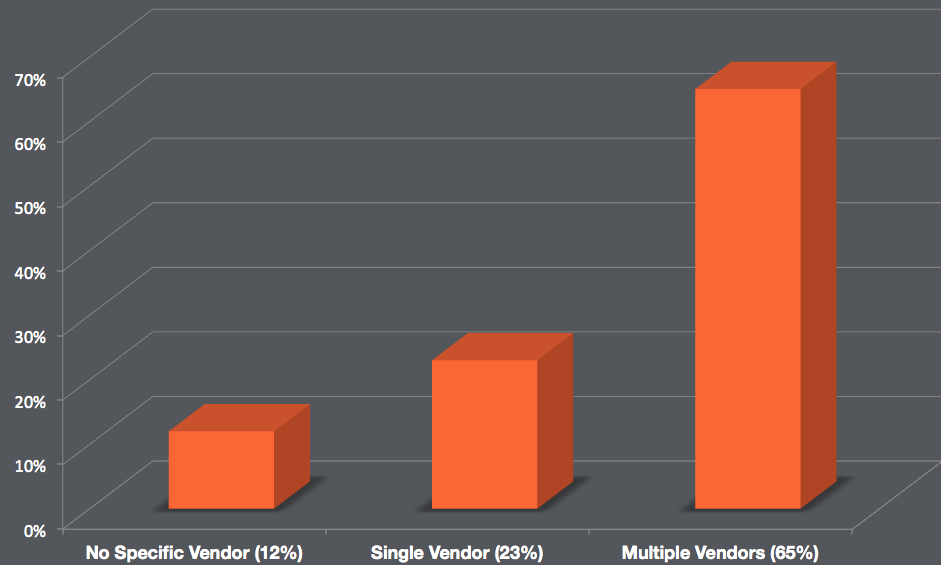
\includegraphics[scale=0.3]{images/graph1.png}
    \end{center}
    \caption{Percentage of companies using multiple vendors}
    \label{fig:graph1}
\end{figure}

According to EMC's report on Global Data Protection Index %[4]
, there exists a direct relationship between the number of vendors that
a company relies on and figures such as IT spending, disruptions, data
loss and the cost of downtime. The more vendors being used, the higher
these damaging numbers climbed. Many companies may feel as if they have
no choice but to use multiple vendors. Often times, backup support is
needed for different operating systems. So, when a company needs support
for both Windows and Linux, they'll often times look to the service of
two vendors; one that supports Windows and one that supports Linux. The
matter of fact is that backup solutions exist that provide support to
more than one operating system. As shown in EMC's report, a single
backup vendor is a financially preferable option for businesses needing
protection over more than one operating system.


\subsubsection{Impact on Disruptions}

Data loss and downtime are a company's worst nightmare. According to
EMC, those organizations using one data protection vendor are the least
likely to experience disruption.

There isn't a significant difference in disruption between companies
using two vendors and those using three or more vendors. However, there
is a significant leap in disruption when compared those using a single
vendor. 54\% of companies using three or more data protection solutions
reported unplanned downtime, while only 42\% of companies using a single
vendor reported downtime. Similarly, 38\% of those using three or more
vendors experienced data loss compared to 24\% of those who use single
vendors.

\subsubsection{Impact on Costs}

Companies who use three or more data protection vendors are being hit
with \$1.66 million in downtime costs. That's more than four times the
amount that it costs those companies who are using just one data
protection vendor (\$0.34 million).


\begin{figure}[t]
    \begin{center}
        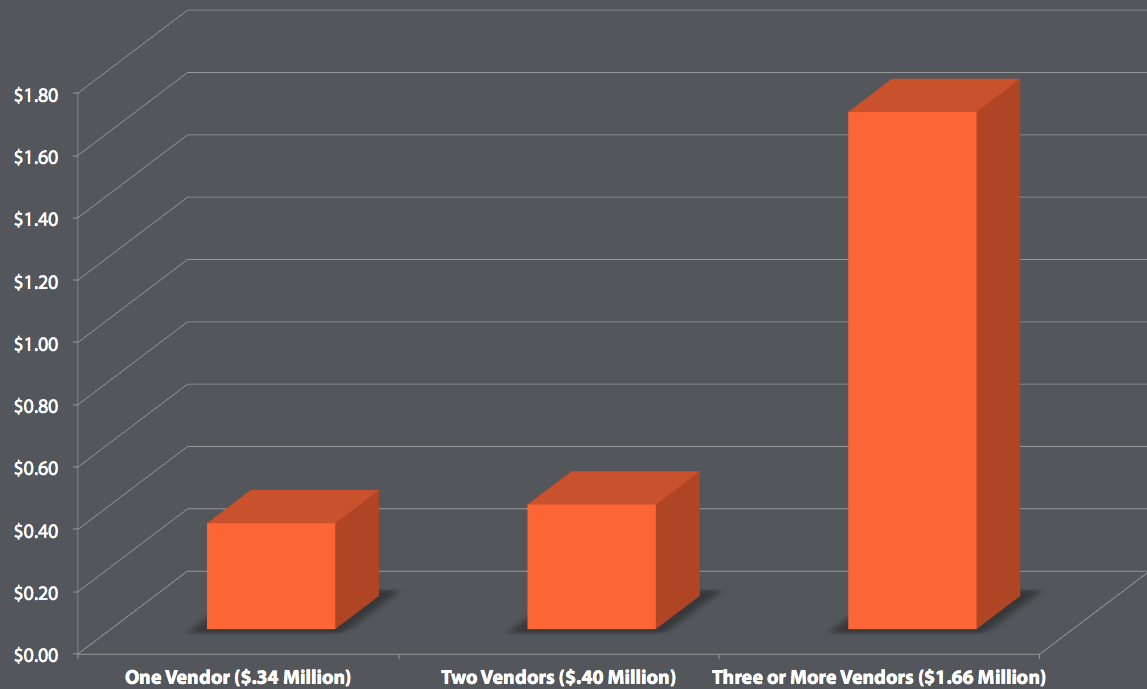
\includegraphics[scale=0.3]{images/graph2.png}
    \end{center}
    \caption{}
    \label{fig:graph2}
\end{figure}

The bottom line is that there is a much greater chance of experiencing
disruption when using multiple data protection vendors, and that using
multiple best-in-breed (highly specialized/cutting edge) solutions can
cause more issues than they claim to solve.


%[4] : http://www.emc.com/collateral/presentation/emc-dpi-key-findings-global.pdf

\section{Future Developments and Requirements}

\subsection{Shift from traditional data structures to ``Big Data''}

As new information is created and handled within the enterprise, IT and
its backup administrators and operators are faced with the challenge of
protecting critical information assets at a much larger scale. Today's
information growth rates have IT organizations at their tipping points.
%[5]
They must ``rethink'' data protection and find the balance between
serving the organization's desire for big data, seeking more value from
the information they create (through data mining and analysis), and the
age old and essential requirement of protecting information from a
disaster, corruption, or a logical or physical system failure.

Meeting the demands of big data backup require both retooling your
approach to data capture and the use of optimization technologies. The
topology of backup targets must evolve from the typical data-centric
model to a more globally dispersed, flexible deployment approach to
achieve better scale and data protection coverage.

\begin{figure}[t]
    \begin{center}
        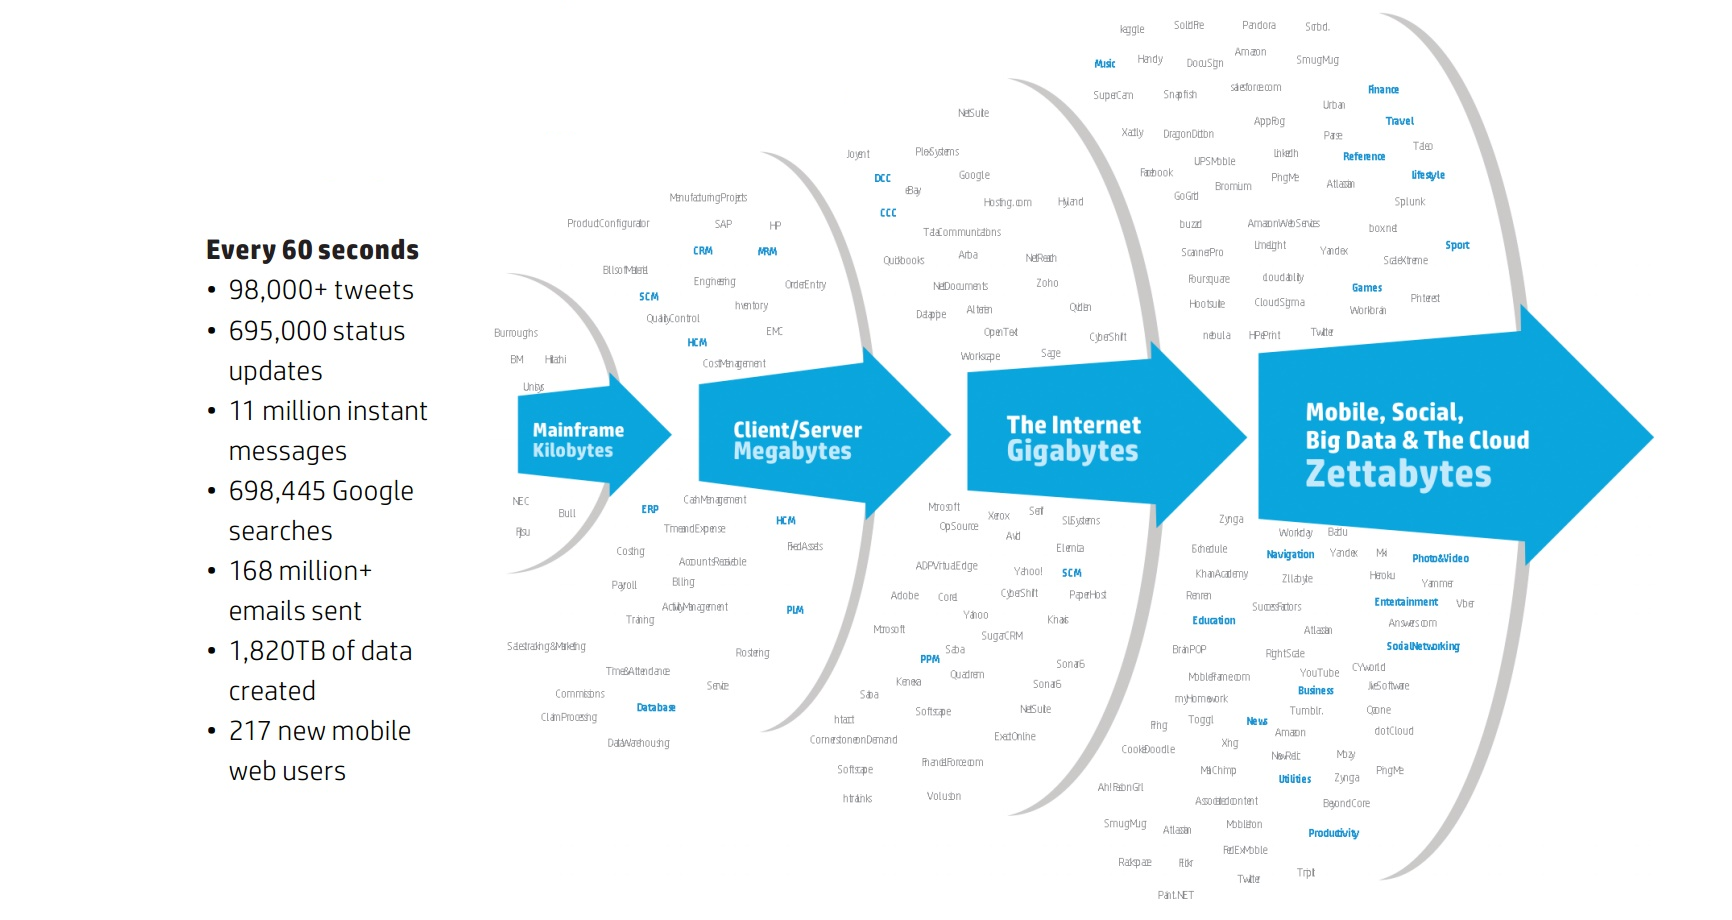
\includegraphics[scale=0.3]{images/graph3.png}
    \end{center}
    \caption{Data volume pace is accelerating}
    \label{fig:graph3}
\end{figure}

Petabyte-size data stores can play havoc with backup windows, and
traditional backup is not designed to handle millions of small files.
Fortunately not all big data information needs to be backed up in the
traditional way. Before considering how to protect your data, you should
decide at what data needs to be protected. Machine-generated data
report data from a database, for instance can be reproduced easier
than it can be backed up and recovered. Compare the cost of protecting
data with the cost of regenerating the data. In many instances, source
data will need to be protected, but any post-acquisition processes may
be cheaper to reproduce than the cost of protecting the data after
manipulation.

Although enterprises have become accustomed to rapid backup data growth,
few are prepared for the avalanche of data that is going to result from
cloud and big data analytics in the coming year and beyond. This data
growth will challenge the capabilities of even the most robust backup
environments. Short-term solutions, solutions with limited scalability,
and solutions that add complexity to the data center will no longer be
viable options.

%[5] : http://esj.com/articles/2012/12/12/big-data-backup-trends.aspx
%[6] : http://h20195.www2.hp.com/V2/GetPDF.aspx/4AA4-6750ENW.pdf

\subsection{Continuous re-evaluation of backup strategy}

Having a clear backup strategy and re-evaluating it according to the
business requirements and needs at least yearly, is necessary to prevent
disaster. The following points need to be addressed and re-evaluated
every time there is a new Business Impact Analysis on backup and
restore.

\begin{itemize}
	\item Address specific business needs. Define a solution for data
		backup as part of a consultative process, while addressing all
		specific business needs.
	\item Conduct TCO analysis. Before moving to a new data backup
		service, a TCO (total cost of ownership) analysis should be done
		to determine the payback period for moving to a new backup
		service. Use a provider that can integrate archives, so you can
		move data sets from a backup plan to an archive plan and
		provides online search and retrieval functionality. And make
		sure your provider has good management processes, good quality
		reporting and a secure facility and connectivity.
	\item Test before provisioning. Put the backup provision in place
		long before you need it.
	\item Encrypt backup data. Security is of prime concern in all forms
		of computing, especially on cloud-based solutions and services.
		To ensure security and privacy always use encrypted backups.
	\item Follow governance and compliance rules. Always make sure to
		follow governance and compliance rules. For example, regulatory
		compliance related to where data may move or be stored when
		different countries or regions are involved, or compliance
		related to retention periods of data. If you are purchasing
		backup service from vendor and a cloud provider then ensure the
		backup service vendor is also following the governing laws for
		that region.
	\item Bulk data import process governance. Data center staff should
		be familiar with process and procedures related to bulk data
		import wherein data is shipped on removable media storage to
		on-premise. This option will be critical when faster data
		recovery is needed for large data backups. In addition customer
		should have in place good governance for data-import process --
		such as who is authorized to receive the removable storage media
		and who is notified.
	\item Backup locally and remotely. Data that is recovered frequently
		should be backed up to both on-premise storage and to cloud
		storage. This is because the on-premise backup assures faster
		recovery, while the off-premise copy can be used for disaster
		recovery purposes.
	\item Backup locally to ensure public accessibility. If the purpose
		of putting data in the cloud is for public accessibility, then
		backup the data locally even before storing in cloud.
	\item Engage multiple vendors. If one can afford it, it is
		recommended to backup very important and critical data to
		multiple vendors to mitigate risks. This gives an extra level of
		safety in case one of the vendors has an outage at a
		business-crucial time.
	\item Ensure data interoperability. Ensure that the backed up data
		can be recovered on premise and/or to another cloud vendor.
\end{itemize}


\subsection{Stress of Uncertainty}

In the end, the stress of uncertainty the last but not least important
factor for the future developments of backup. With key information about
backups divided on multiple, individual systems, IT staff have more
uncertainty to deal with and a harder time making holistic, informed
decisions about their company-wide backup environments.

A solution should be chosen that enables IT data managers to get fast,
accurate information on the status of their entire backup environment.
Robust dashboard functionality can not only enable a single
administrator to manage more backup data, it can also enable them to
reduce inefficiencies in their backup environment, plan for future
capacity needs, and ensure restore Service Level Agreements (SLAs) are
achievable.

While the impact on morale is harder to quantify, the human costs of
sprawl can quickly affect the bottom line with increased staff turnover,
low staff productivity, increased overtime. By consolidating backups and
automating backup tasks, companies can free key IT staff for more
productive and more gratifying work but most importantly achieve their
mission; meeting their SLAs and reducing the business risk of data loss
and downtime.

Scalable, enterprise-class systems also provide a tighter level of
management control and reporting to ensure IT departments get the most
value from their backup investment and more accurate planning for future
needs.
